\newpage % Zaleca się otwieranie rozdziału od nowej strony.


\section[Wstęp]{Wstęp}

% Co znajdzie sie w pracy a bardziej jaki zrobic wstęp.
Szybkosc, dokladnosc ruchu i wysoka nośność manipulatoów robotycznych. Czy można mieć wszystko?
Manipulatory rownoległe zdają się spełniać wszystkie te wymagania, gdy nie jest potrzebny daleki zasięg ramion robotycznych.
Najbardziej popularnymi przedstawicielami tej grupy są roboty delta, które dzięki wysokiej szybkości operacyjnej są wykorzystywane w systemach pakujących, ale oferują zazwyczaj tylko cztery stopnie swobody. Szerszy obszar zastosowań można osiągnąć dodając do projektu dodatkowe stopnie swobody. Przykładem takiego manipulatora równoległego z sześcioma stopniami swobody jest konstrukcja Gougha-Stewarta, zwana potocznie hexapodem lub po prostu platformą Stewarta.

Celem mojej pracy inżynierskiej jest wykonanie konstrukcji i zaprogramowanie manipulatora równoległego o sześciu stopniach swobody.
% pisac ze mcu bedzie STM i ze serwa i ze mialo byc tanio?
Gotowe urządzenie następnie wykorzystano do sterowania położeniem kulki na talerzu platformy za pomocą regulatora PID i odczytów z rezystancyjnego panelu dotykowego.


%Szeregowe i rownolegle lancuchy kinematyczne???


\begin{figure}[!h]
    \label{fig:anzelm}
    \centering 
    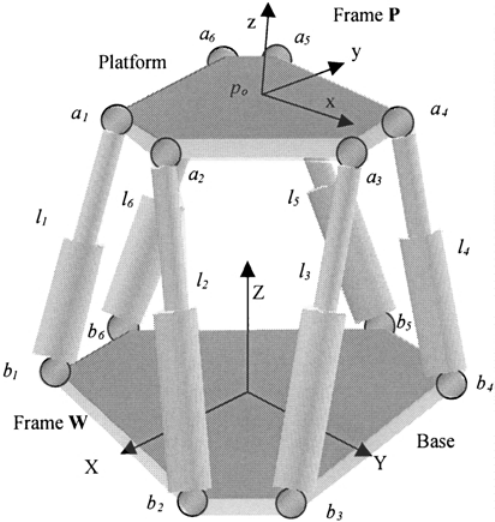
\includegraphics[width=0.4\linewidth]{img/stewart_researchgate_net.png}
    \caption{Budowa mechaniczna platformy Stewarta}
    % \captionsource{Źródło: }{http://www.researchgate.net}
\end{figure}


\subsection{Historia konceptu Platformy Stewarta}
% [http://www.parallemic.org/Reviews/Review007.html]

W roku 1954 dr. Eric Gough zaprojektował i skonstruował pierwszy hexapod - uniwersalna maszyne do testowania opon dla angielskiej fabryki w Birmingham.
Skąd więc pochodzi nazwa platforma Stewarta? W 1965 roku D. Stewart opublikował artykuł, w którym zaprojektował symulator lotu. Popularność jego artykułu w społeczeństwie akademickim spowodała przejęcie nazwy manipulatora jako platforma Stewarta, czasami tylko nazywaną platformą Gougha-Stewarta. 
W dniu dzisiejszym Platforme Stewarta należy rozumieć jako manipulator składający się z mobilnego talerza górnego przymocowanego do nieruchomej bazy za pomocą sześciu  niezależnych kinematycznie względem siebie nóg o zmiennej długości.

\begin{figure}[!h]
    \label{fig:anzelm}
    \centering
    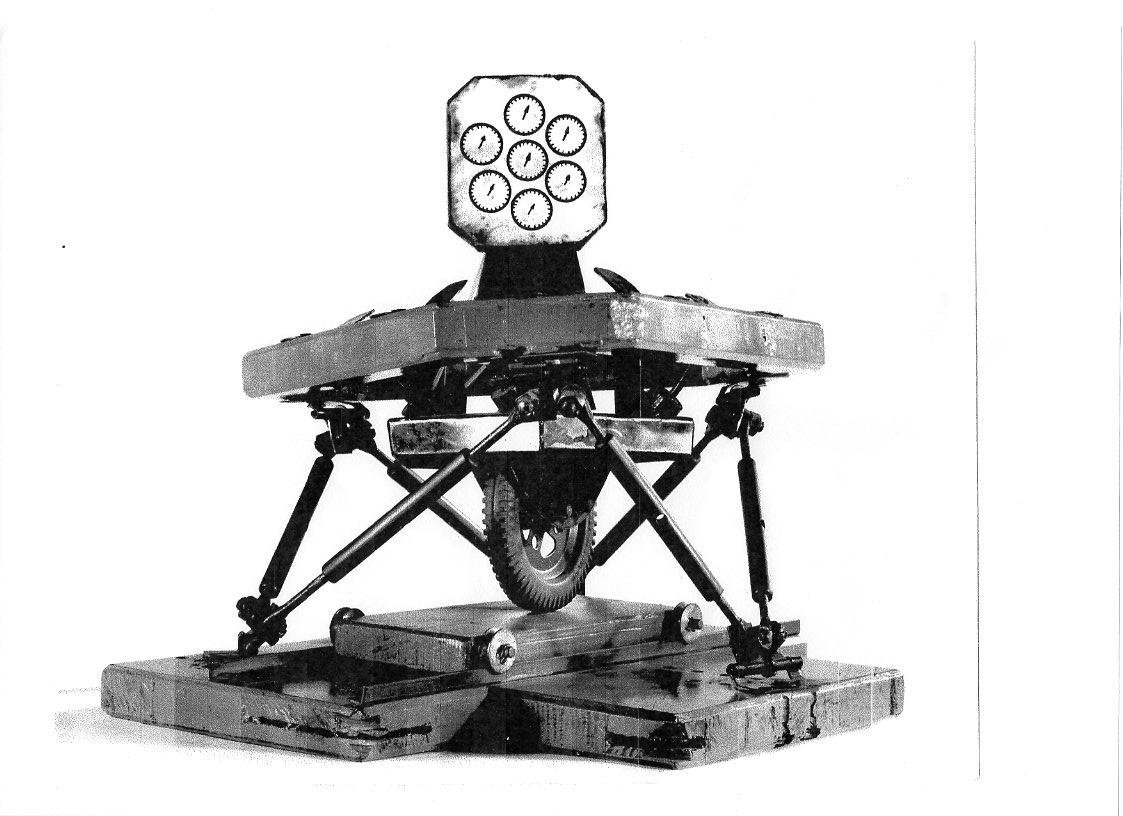
\includegraphics[width=0.5\linewidth]{img/GoughPlatform.jpg}
    \caption{1954 - pierwszy hexapod autorstwa dr. Erica Gougha.}
\end{figure}


% [Stewart, D. (1965–1966). "A Platform with Six Degrees of Freedom". Proceedings of the Institution of Mechanical Engineers. 180 (1, No 15): 371–386. doi:10.1243/pime_proc_1965_180_029_02.]



\subsection{Czy 6 DOF to coś specjalnego?}

Wykorzystanie sześciu kinematycznie niezależnych aktuatorów w tej konstrukcji, sprawia że talerz górny platformy, jako ciało sztywne, moze się poruszać swobodnie w przestrzeni 3D względem podstawy.
Oznacza to, że fizyczny punkt na talerzu może poruszać się w osi X, Y, Z, a także wykonywać wokół nich rotacje.
Wiąże się to z tym, że położenie platformy można opisać za pomocą sześciu zmiennych, trzech opisujących przesunięcia na osiach i trzech opisujących rotacje wokół tych osi.

\begin{figure}[!h]
    \label{fig:anzelm}
    \centering
    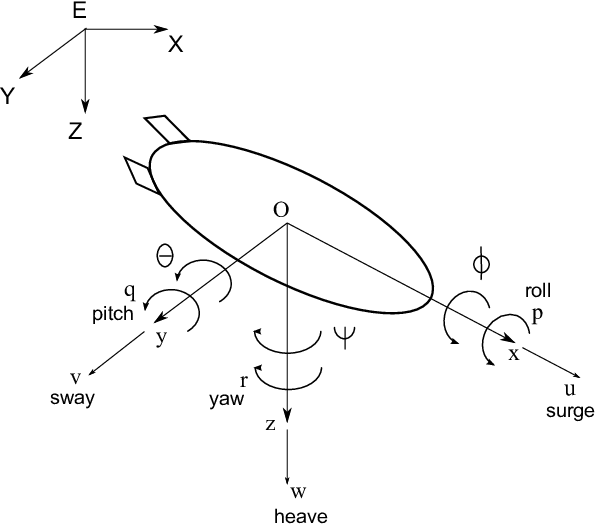
\includegraphics[width=0.5\linewidth]{img/6-DOF-reaserchgate.png}
    \caption{Przedstawienie wolności ruchu przy 6 stopniach swobody.}
    % \captionsource{Źródło: }{https://www.researchgate.net/publication/314264419}
\end{figure}


\subsection{Czym się cechują takie urządzenia? Po co to komu?}
% Rózne mechaniczne designy: https://repository.up.ac.za/bitstream/handle/2263/25175/01chapter1.pdf?sequence=2

Mimo wielu konceptów konstrukcyjnych na uzyskanie manipulatora równoległego o 6 stopniach swobody wykorzystanie konstrukcji zapoczątkowanej przez dr. Gougha przynosi wiele korzyści. 
System taki cechuje się szerokim zakresem ruchów, dużym udźwigiem, a także precyzją ruchu. Dokładność ta spowodowana jest sztywnością całego urządzenia, gdzie zastosowane elementy mechaniczne mają mniejszą skłonność do pojawienia sie sił gnących, jak np. przy szeregowym łańcuchu kinematycznym, którymi są robotyczne ramiona antropomorficzne.

% Engineers and researchers have examined many variants of the Stewart Platform. Most variants have six linearly actuated legs with varying combinations of leg-platform connections. Of the many types of motion control platforms, the Stewart Platform is useful to study because it is a widely accepted design for a motion control device. This is largely because of the system's wide range of motion and accurate positioning capability. It provides a large amount of rigidity, or stiffness, for a given structural mass, enabling the Stewart Platform system to provide a significant source of positional certainty.

% The design of the Stewart Platform supports a high load-carrying capacity. Because of the design, the legs carry compression and tension forces, and will not succumb to the undesirable bending force found in other designs. The six legs are spaced around the top plate and share the load on the top plate. This differs from serial designs, such as robot arms, where the load is supported over a long moment arm.



\subsection{Czy jest to faktycznie wykorzystywane? Dlaczego tak/nie?}
% symulator lotu, robot hirurgiczny, nakierowywanie anten, platformy do ladowania rakiet
Układ kinematyczny Stewarta początkowo został zaprojektowany jako maszyna do badania opon, potem jednak docelowo został wykorzystywany jako korpus symulatorów lotów, w których to sytuacjach wykorzystywana jest zaleta wysokiej siły nośnej. 
Nie oznacza to jednak, że konstrukcja nie ma więcej zastosowań. 
Ze względu na swoją wysoką prezyzje, taki manipulator może być wykorzystywany do przeprowadzania operacji hirurgicznych. 
Z kolei szeroki jego zakres ruchów może znaleźć zastosowanie przy ustawianiu anten radioteleskopów, czy paneli słonecznych.



% \begin{figure} [H]
% \centering
% \begin{tabular}{ccc}
% 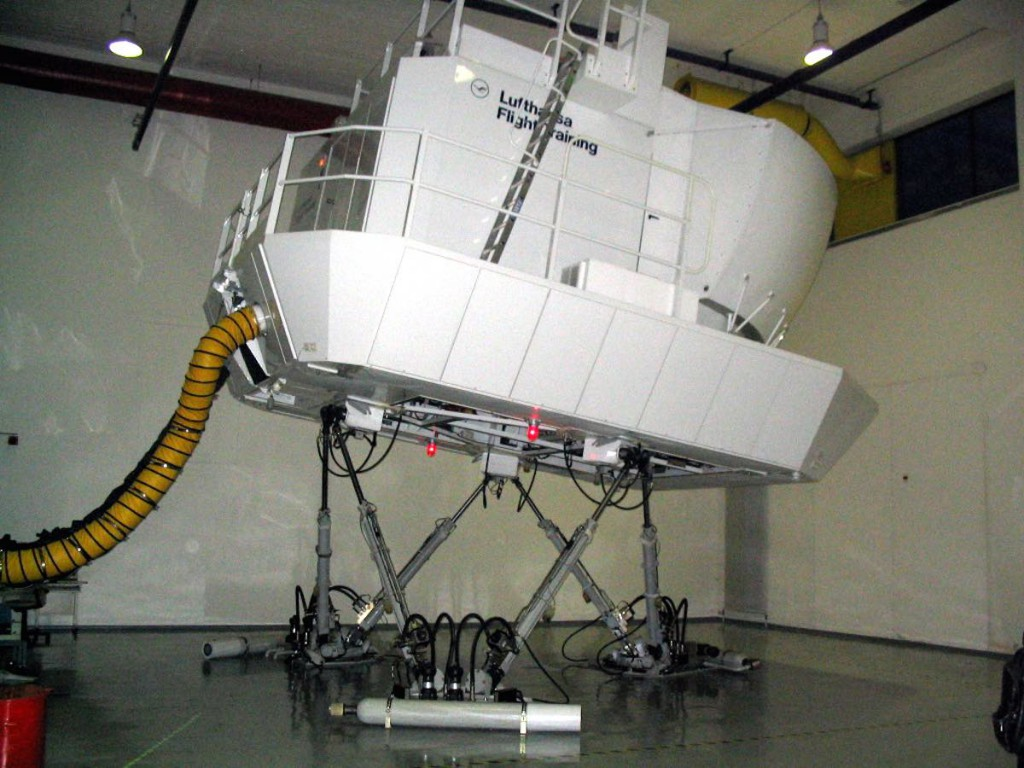
\includegraphics[width=0.3\linewidth]{img/Boeing_737_Full_Motion_Flight_Simulator-1024x768.jpg} &
% 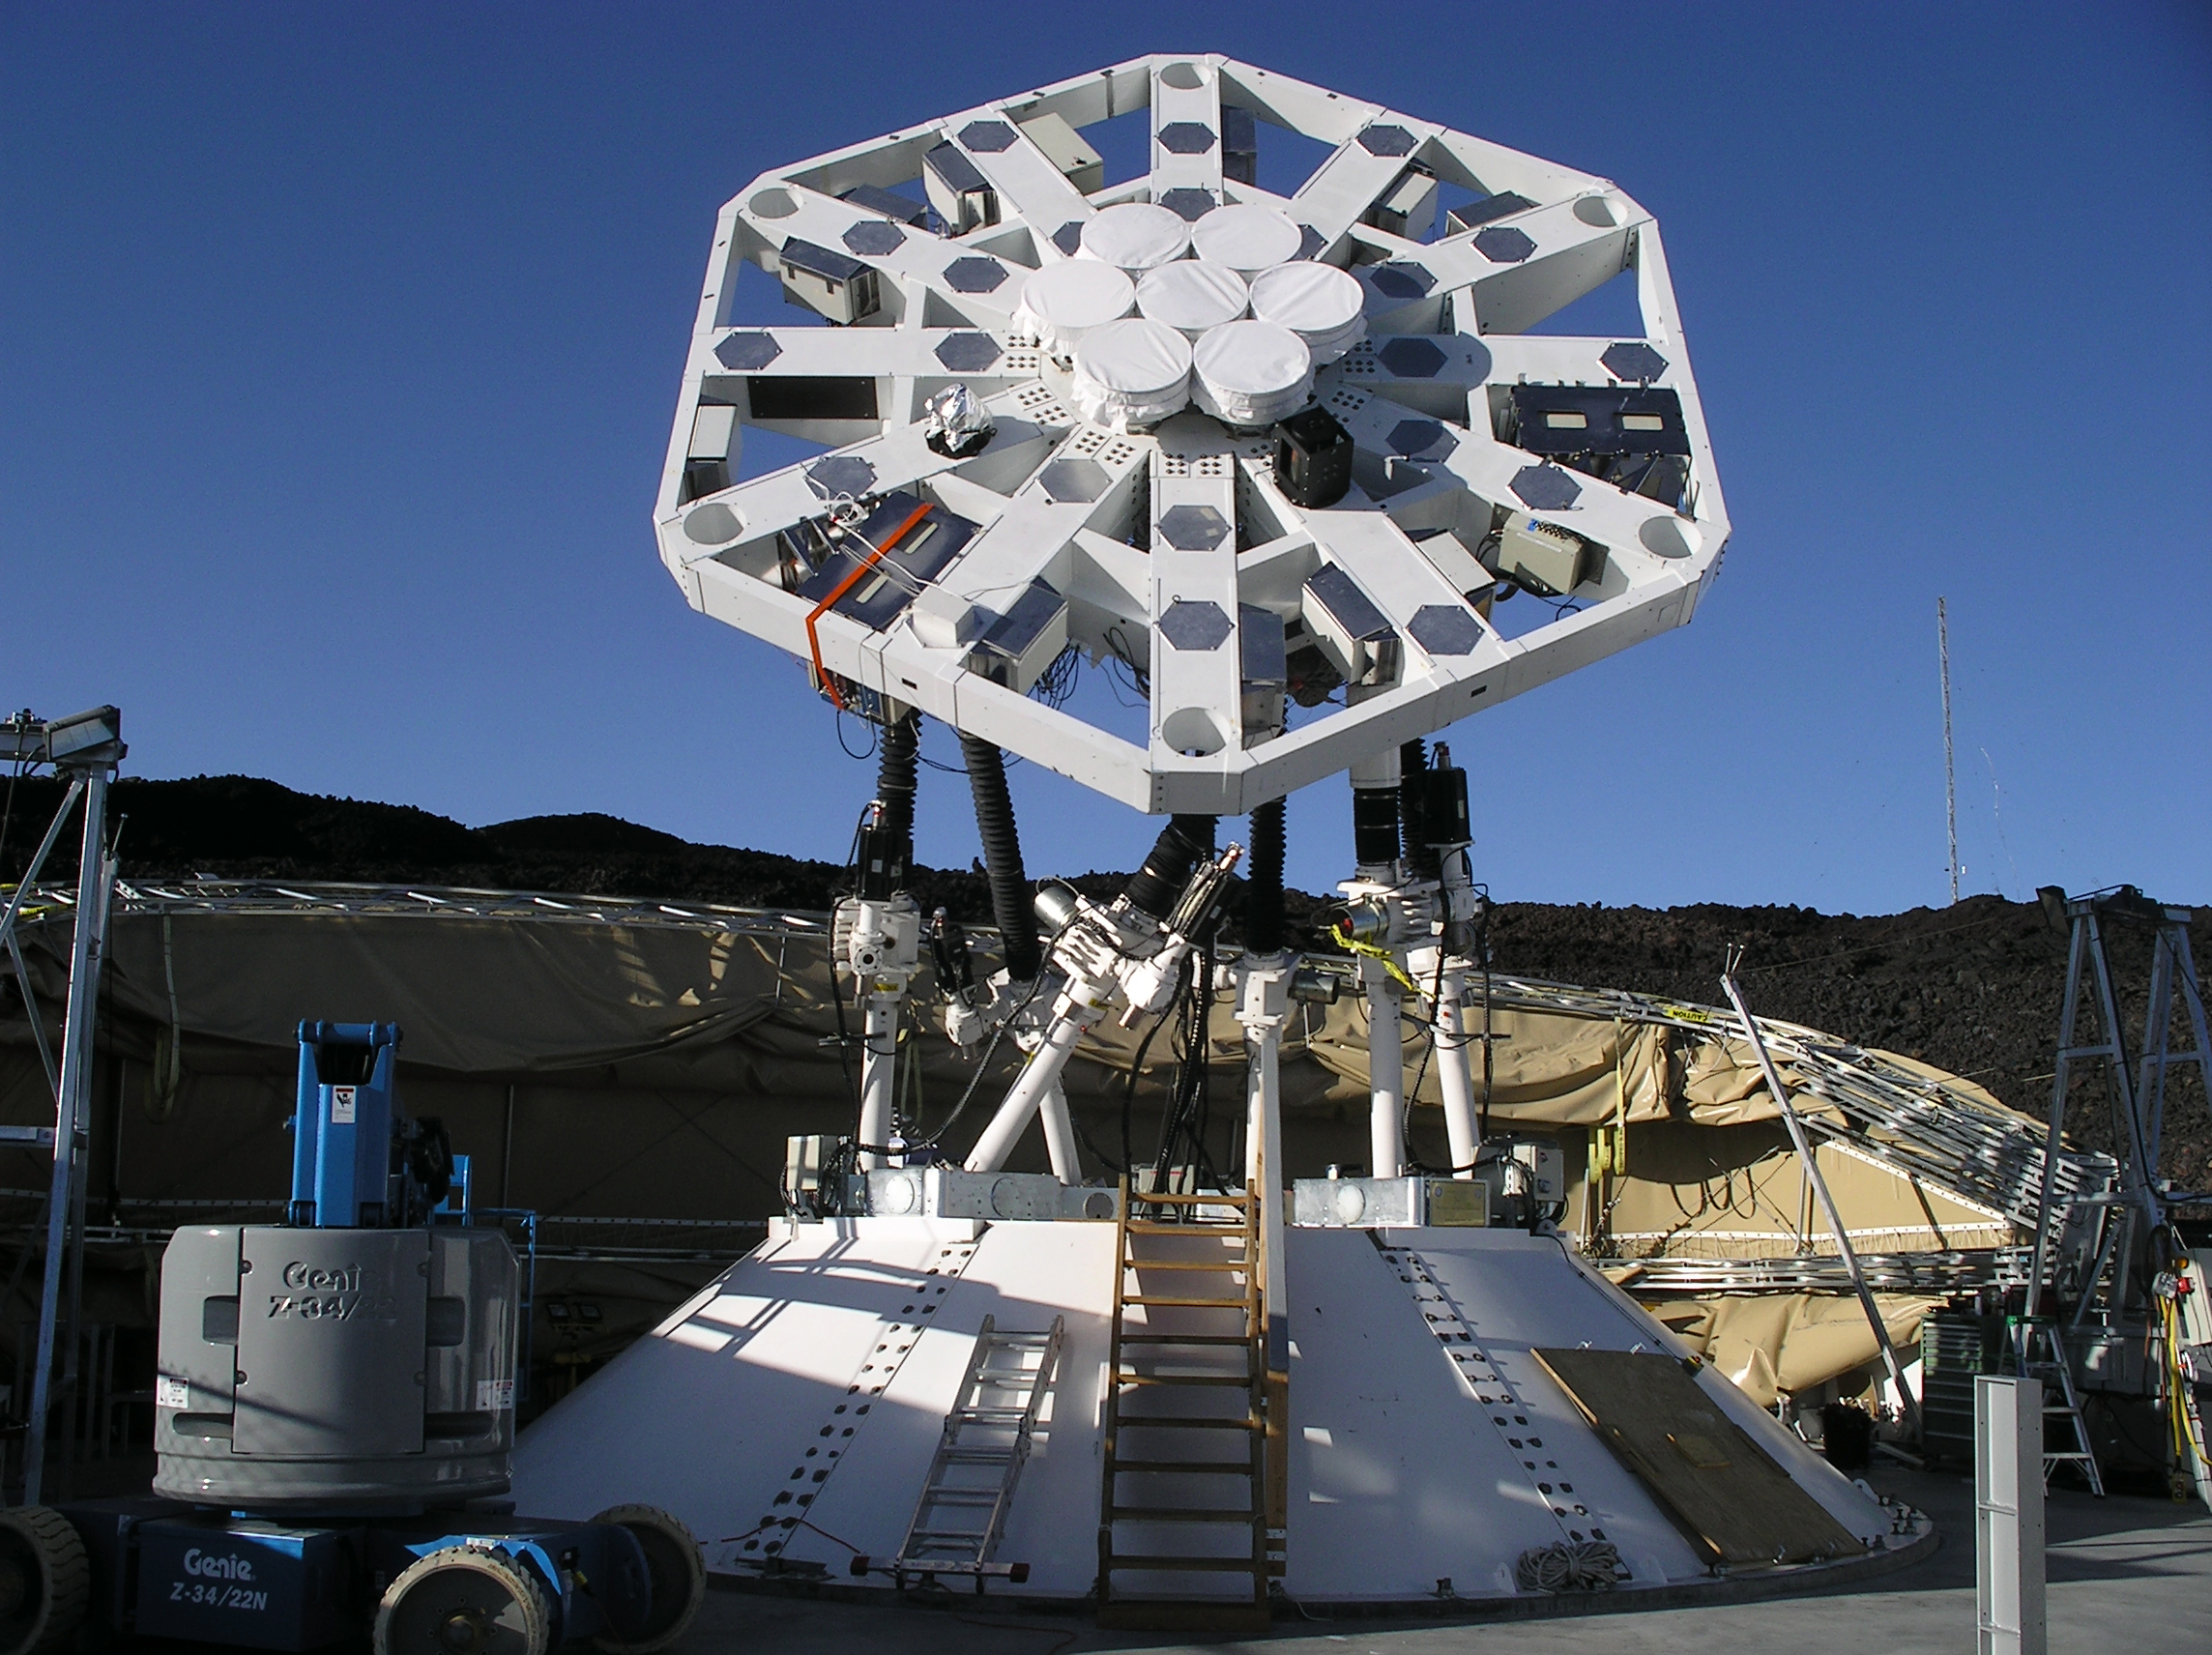
\includegraphics[width=0.3\linewidth]{img/amibia_telescope.jpg} &
% 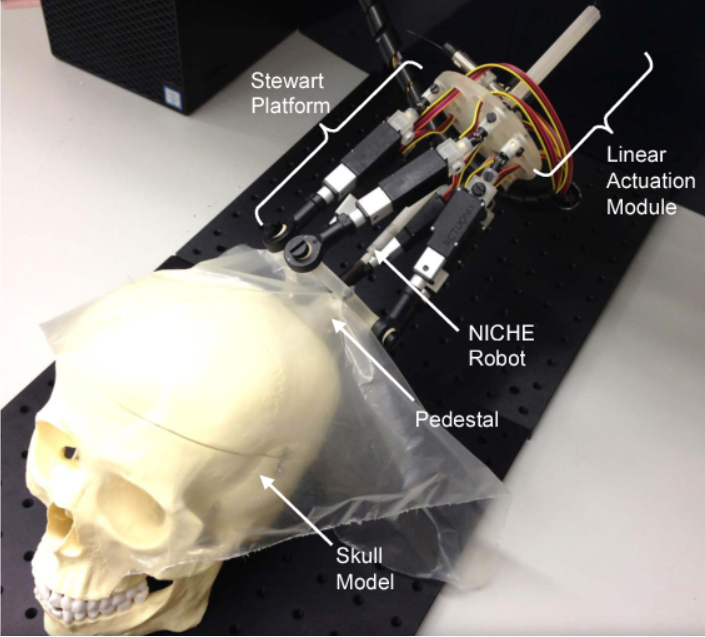
\includegraphics[width=0.3\linewidth]{img/medical_surgery_stewart.png} \\
% \textbf{a)Symulator lotu}  & \textbf{b) Teleskop} & \textbf{c) Robot neurochirurgiczny.}  \\[6pt]
% \end{tabular}
% \caption{ 
% \textbf{a)} Symulator dla samolotu Boeing 737.\\
% \textbf{b)} Teleskop YTLA (dawniej AMiBA) badający mikrofalowe promieniowanie tła przestrzeni kosmicznej.\\
% \textbf{c)} Robot neurochirurgiczny mający na celu zredukowanie inwazyjności operacji.}
% \label{fig:Name}
% \end{figure}

% The Stewart Platform was originally designed in 1965 as a flight simulator, and it is still commonly used for that purpose. Since then, a wide variety of applications have benefited from this design. A few of the industries using the Stewart Platform design include aerospace and defense, automotive, transportation, and machine tool technology, who use the platform to perform flight simulation, handle vehicle maintenance, and design crane hoist mechanisms. The Stewart Platform design is also used for the positioning of satellite communication dishes and telescopes and in applications such as shipbuilding, bridge construction, transportation, and as a drilling platform on the Lunar Rover.



